%
% konzertsaal.tex
%
% (c) 2023 Prof Dr Andreas Müller
%
\begin{figure}
\centering
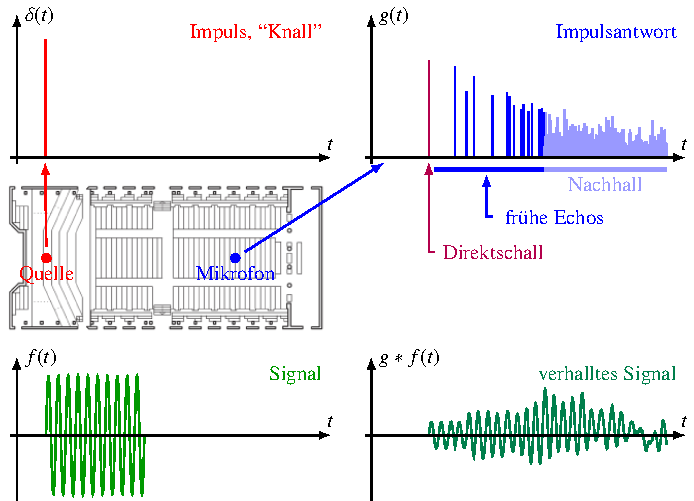
\includegraphics{chapters/030-gruppen/images/konzertsaal.pdf}
\caption{Echos und Nachhall in einem Konzertsaal.
Eine einzelner Impuls von einer Quelle (rot) führt beim Mikrofon
zu einer komplizierten Impulsantwort $g(t)$ bestehend aus
dem Direktschall, den frühen Echos und dem Nachhall.
Ein beliebiges Signal $f(t)$ (grün) wird beim Mikrofon als $g*f(t)$
aufgenommen.
\label{buch:gruppen:faltung:fig:konzertsaal}}
\end{figure}
